\documentclass[12pt]{scrartcl}
\usepackage[german]{babel}
\usepackage{graphicx}
\usepackage{subcaption}
\usepackage[latin1]{inputenc}
\usepackage[T1]{fontenc}

\usepackage{color}
\usepackage[linkcolor=black, urlcolor=black, citecolor=dblue,
breaklinks, bookmarks, colorlinks]{hyperref}

\begin {document}

\hspace{-0.4cm}\huge \textbf{Freeze Me! - Dokumentation}\vspace{3pt}\\\Large A Media Processing Project \vspace{14pt}\large 

\noindent
\textbf{Stand:} 28.02.2023 \\

\vspace{3pt} \normalsize Gruppe: 
Jan Rekemeyer, Iskander Yusupov und Hendrik Finke

\section{Motivation}
Da das Ziel des Projekts darin bestand, ein Softwareprodukt zu erstellen, entschied sich die Gruppe, eine Motivation im Marketingformat zu erstellen.\\Gl\"uckliche Momente lassen sich in einem Foto festhalten, das dann verschenkt werden kann. Aber was tun mit den gl\"ucklichen Momenten, die auf Video festgehalten wurden? Mit diesem Ansatz suchte die Gruppe nach M\"oglichkeiten, ein Video so in Form eines Bildes festzuhalten, dass dieses sp\"ater beispielsweise als gerahmtes Geschenk pr\"asentiert werden k\"onnte.
Eine weitere Inspiration f\"ur unsere Gruppe waren Videos mit viel Dynamik. Sport, Tanz, aber auch Tiktok-Challenges enthalten viel Bewegung. Beim Fotografieren von sich bewegenden Objekten erzeugt die Einstellung einer Langzeitbeleuchtung den Effekt einer \glqq eingefrorenen\grqq  Bewegung. Diese Fotos haben ihre eigene \"Asthetik und unsere Gruppe wollte versuchen, diesen Effekt mit den im Modul erlernten F\"ahigkeiten zu reproduzieren.

\section{Zielsetzung}Unser Projekt haben wir der folgende Zielsetzung gewidmet: \\
\textit{Wir entwickeln ein Programm, welches es erm\"oglicht aus einem Video ein Bild zu erzeugen, welches die Bewegungsdynamik des Videos \"asthetisch einfasst und dabei den Eindruck fortw\"ahrender Bewegung erh\"alt.}

\section{Langzeitbelichtung - Inspirationsquelle} %Erstmal Hendriks Sektion
\subsection{Motivation}Das in den Er\"offnungsfolien gezeigte Bildmaterial erinnerte uns in Teilen doch recht stark an eine klassische
Langzeitbelichtung, wie
man sie aus der Analogfotografie oder der Fotographie mit DSLRs oder DSLMs kennt. Daher stellten wir uns die Frage, wie man dieses Konzept digital nachtr\"aglich unter Zuhilfenahme eines Videos anstelle eines Fotos reproduzieren kann.\\
 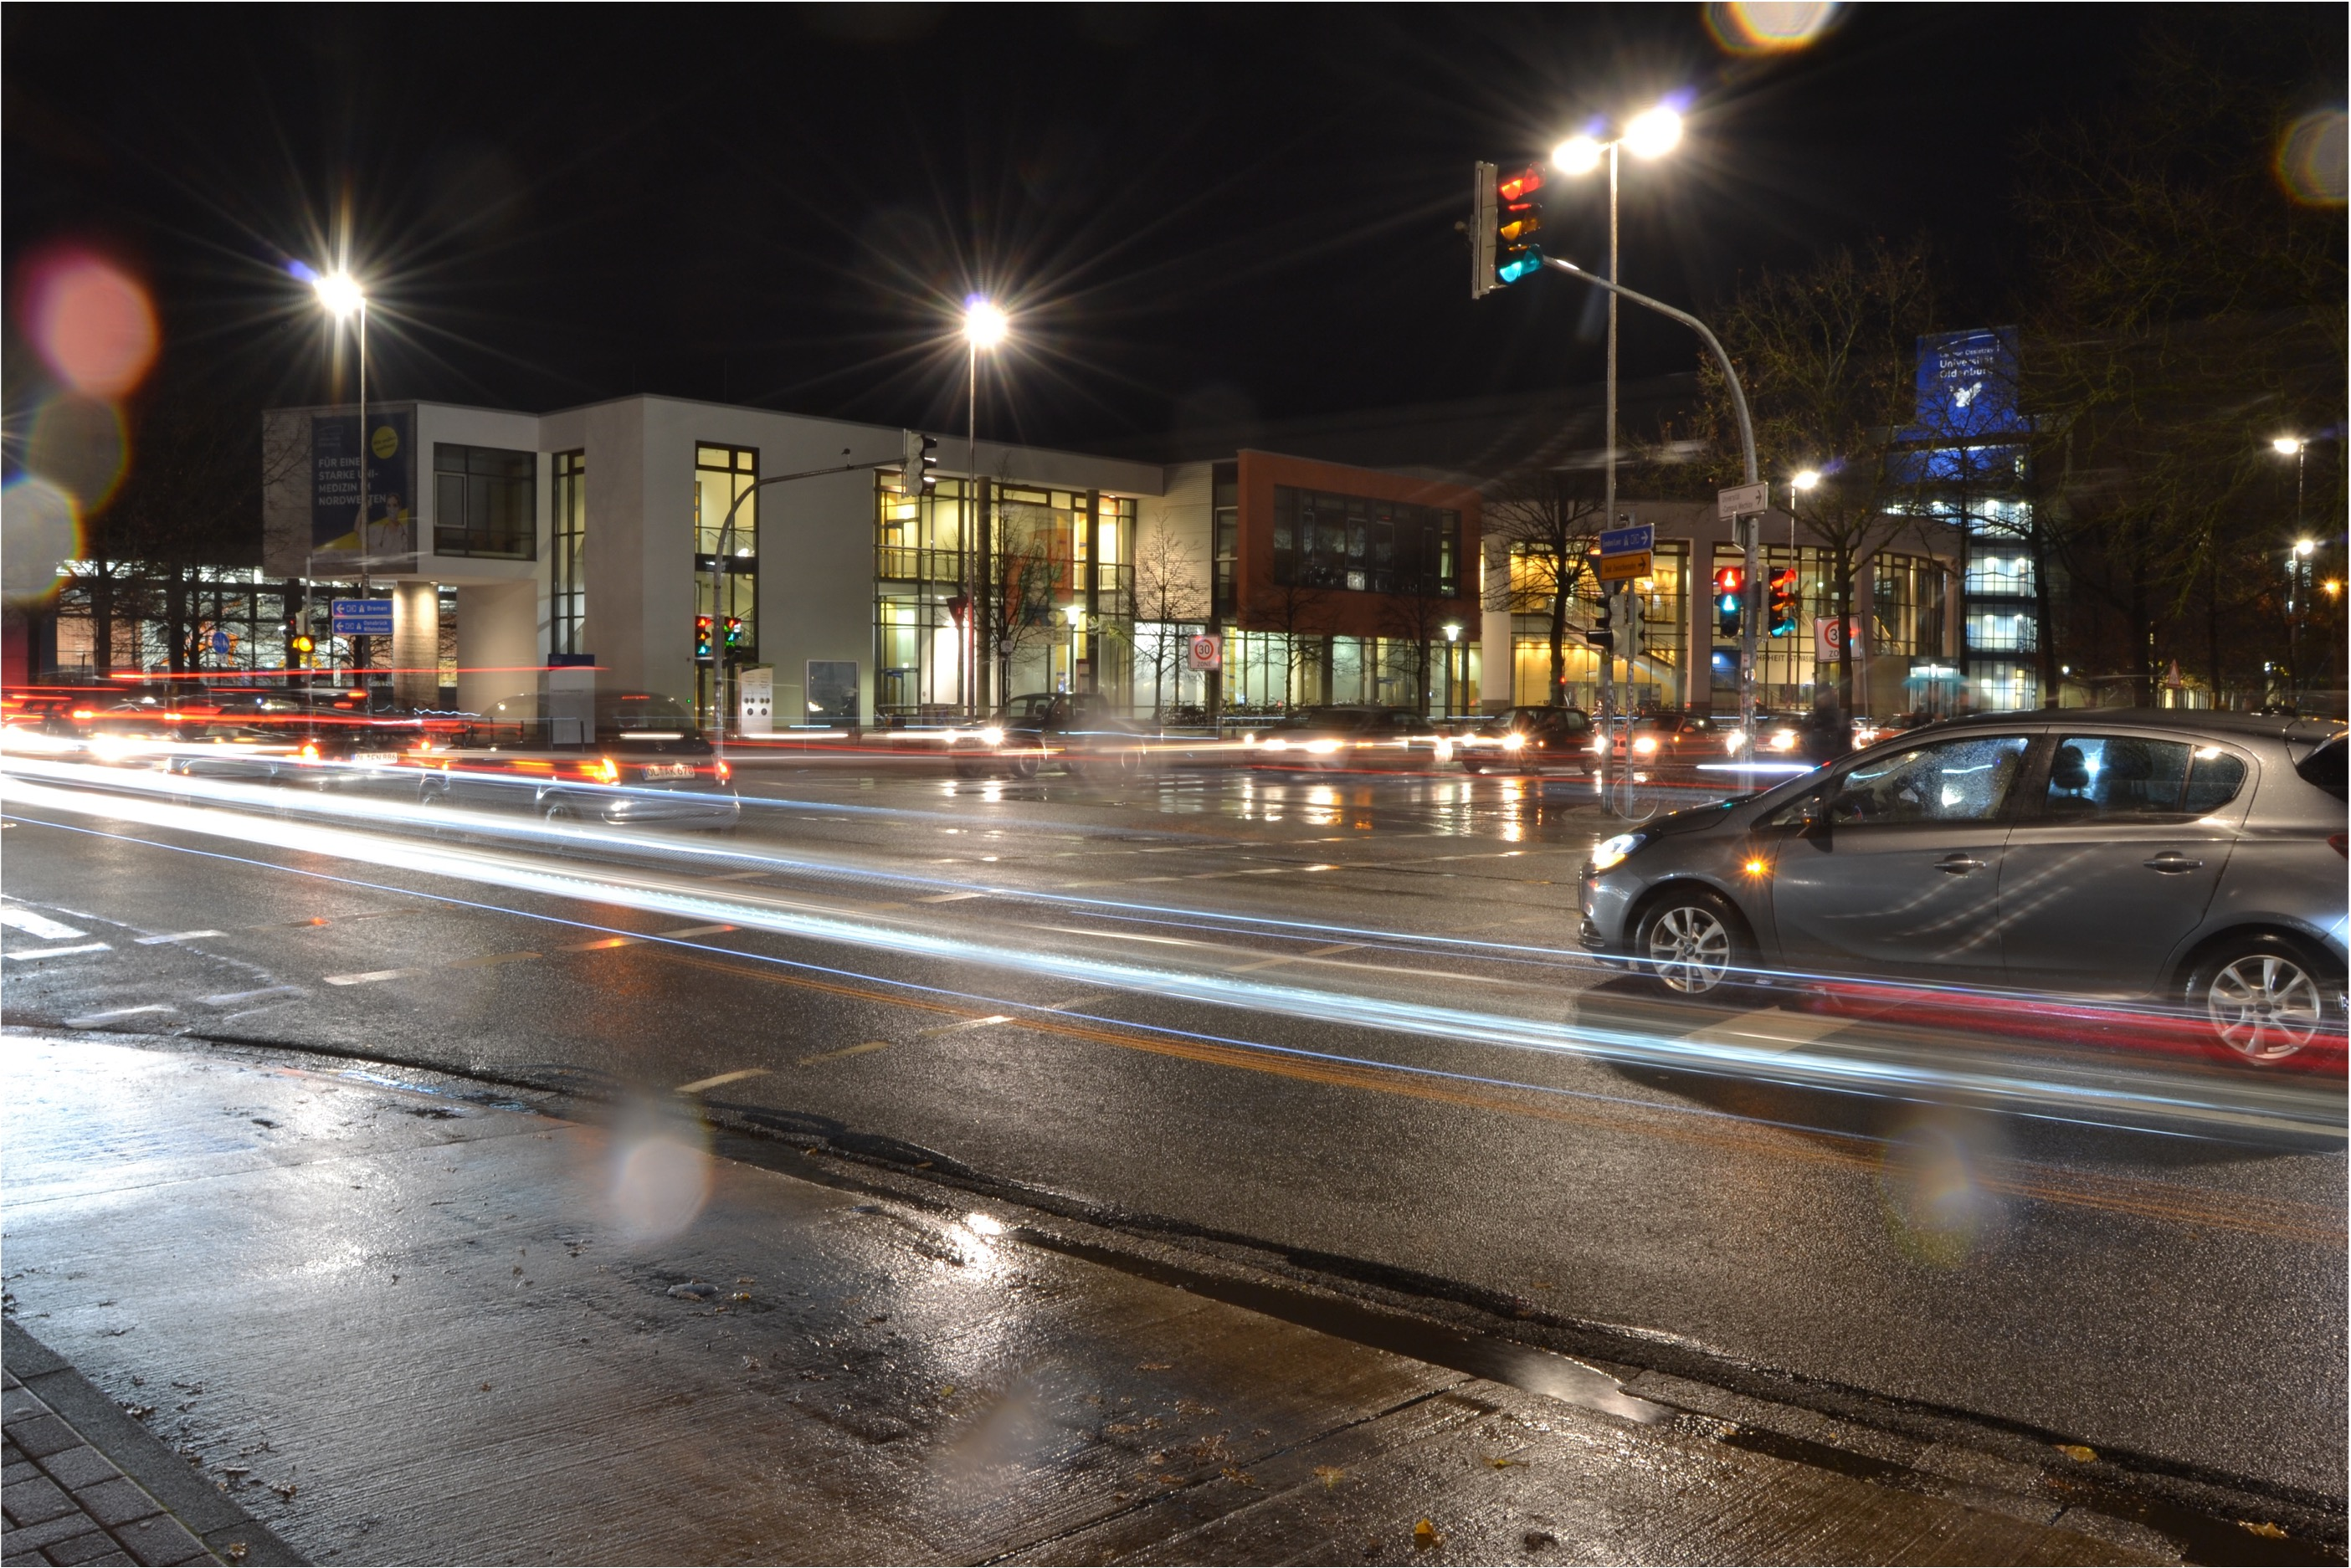
\includegraphics[width=\textwidth]{media/lzb}\\
\subsection{Funktionsweise}Der Ansatz, den wir hierbei Verfolgt haben ist relativ trivial. \"Ahnlich wie klassiche Filter den
Inhaltswert eines Pixels anhand einer ggf. faktorisierten Durchschnittsberechnung mit den umliegenden Pixeln berechnet tun wir ebendieses - jedoch mit den Pixeln gleicher Koordinaten auf anderen Videoframes. Zu diesem Zwecke werden Videos Frame f\"ur Frame betrachtet und dann Pixel f\"ur Pixel in ihre jeweiligen 3 Farbkomponenten zerlegt. Im folgenden wird der Durchschnittswert der Farbwerte errechnet und somit eine Art Langzeitpixel erzeugt, deren Summe das k\"unstlich Langzeitbelichtete Bild ergibt.\\
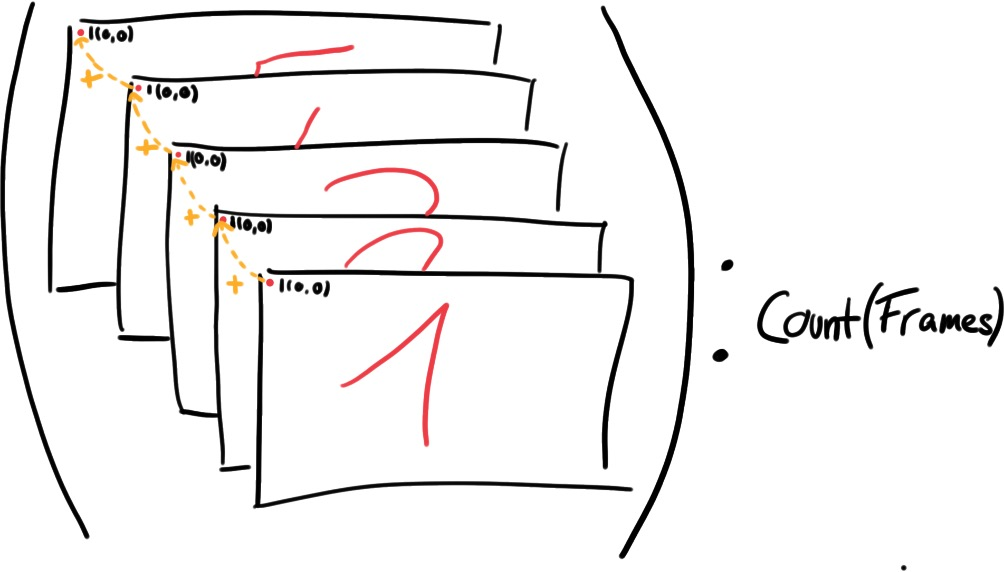
\includegraphics[width=0.6\textwidth]{media/funclzb}
 \subsection{Resultate}Die Resultate waren abh\"angig vom eingegebenen Video durchaus vielversprechend. Ein von uns anf\"anglich eigens erstelltes Video von der Kreuzung der Ammerl\"ander Heerstra{\ss}e mit dem Uhlhornsweg resultierte in einem mehr oder minder matschigen Bild. Das Ergebnis des Contemporary Dancers hingegen war schon erstaunlich dicht an den Hintergrunderscheinungen der Fotos in den Veranstaltungsfolien. Auch das TikTok Video mit dem Sprung resultierte in einem relativ ansehnlichen Ergebnis. Da dieser Ansatz somit der erste nennenswerte Schritt in die Richtung des Gesamtzieles war wurde er beibehalten und die Langzeitbelichtung wurde somit Grundkomponente unseres Projektes.\\
 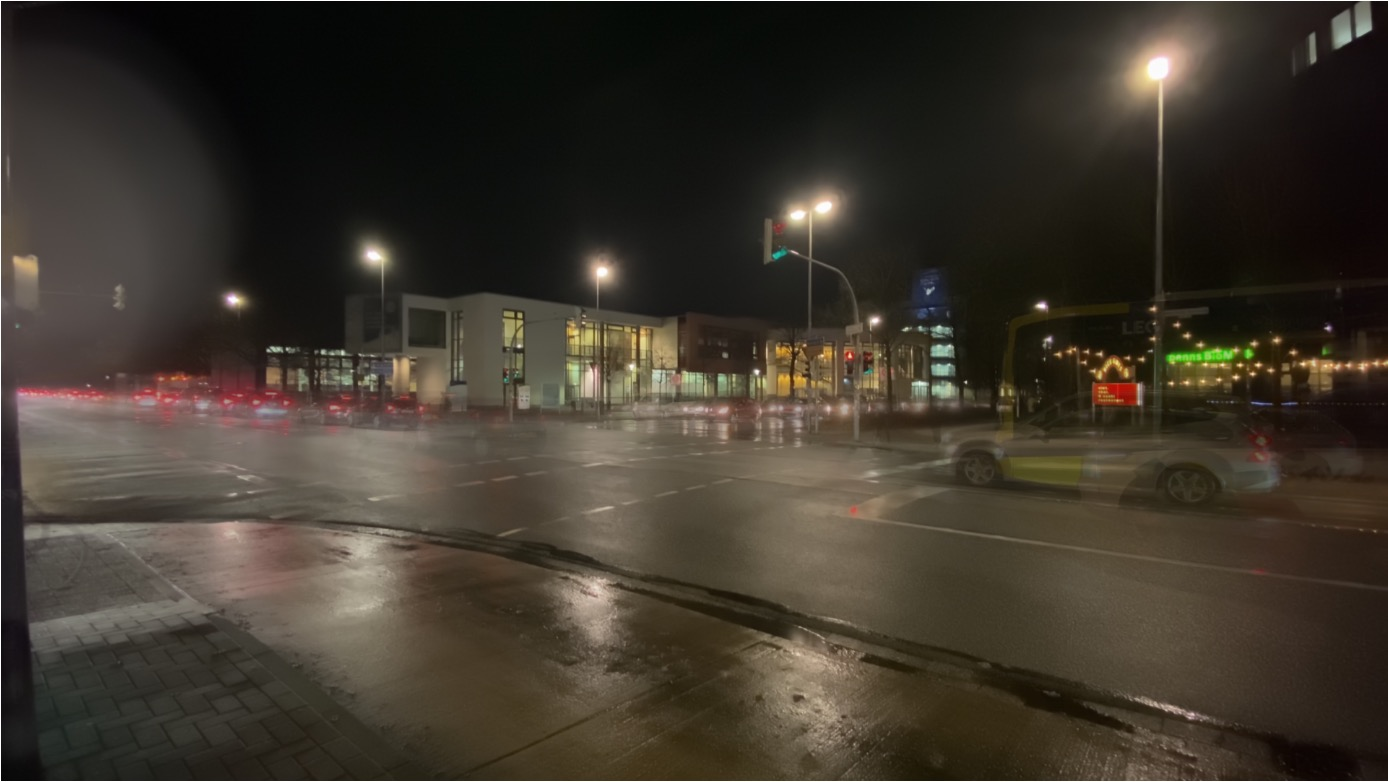
\includegraphics[width=\textwidth]{media/artlzb}
% Anforderungsanalyse

% Langzeitbelichtung
% -> Motivation, Theorie, Codebeschreibung, Resultate

\section{Grabcut mit Thresholding}
\subsection{Motivation}
Mit der Langzeitbelichtung haben wir einen \"asthetischen Schleiereffekt, der im Video stattfindenden Bewegung, geschaffen. Dieser Schleier muss aber noch in ein Bild eingearbeitet werden, sodass der Effekt entsteht, dass die Bewegungen innerhalb eines Videos in Abh\"angigkeit zu einem Hauptbild, einem Frame des Videos, sind. Um dieses zu bewerkstelligen, muss die Langzeitbelichtung mit seinem Schleiereffekt sich um die bewegende Objekte des gew\"ahlten Frames legen. Die sich bewegenden Objekte trennen wir vom Rest des Bilds durch den Foreground Detection Algorithmus GrabCut und verarbeiten diese rausgeschnittenen Bilder zu einer Maske mittels Thresholding.
\subsection{Theorie}
Der GrabCut Algorithmus sch\"atzt innerhalb eines definierten Bereichs die Farbverteilung des Vorder- und Hintergrund mithilfe eines Gau{\ss}schen Mischungsmodells. Die daraus resultierenden Pixeletiketten werden zu einem Graphen zusammengesteckt, in Abh\"angigkeit von der Anzahl verbundener Pixelregionen, die das gleiche Pixeletikett besitzen, sodass eine auf Graphenschnitt basierende Optimierung auf diesem Graphen durchf\"uhrt werden kann. Das genannte Verfahren kann mit dem resultierenden Ergebnis wiederholt werden bis zur Konvergenz. % https://en.wikipedia.org/wiki/GrabCut
\subsection{Codebeschreibung}
Zu Beginn wird das Video, welches den Schleiereffekt erhalten soll, bis zum Ende gespult, der letzte Frame ausgelesen und als separate JPG-Datei abgespeichert. Danach werden Hilfsvariablen f\"ur das Hintergrundmodel, Vordergrundmodel, Maske und auszuschneidende Rechteck initialisiert. Der GrabCut-Algorithmus, der mit den Hilfsvariablen benutzt wird, ist von OpenCV. Der GrabCut-Algorithmus generiert eine Maske, welche mit dem letzten Frame des Videos verrechnet wird, sodass ein Bild von den sich bewegenden Objekten mit sonst schwarzem Hintergrund generiert wird. Die farbigen sich bewegenden Objekte werden dann noch mittels Thresholding wei{\ss} eingef\"arbt, sodass die daraus resultierende Maske beim Zusammenf\"uhren des Schleiereffekts und des letzten Frames verwendet werden kann. Nach der Zusammenf\"uhrung bleibt das finale Bild.
\subsection{Resultate}
Dieser Bildverarbeitungsschritt beschr\"ankt sich derzeit auf das aus unseren Pr\"asentationen bekannte Video vom \textit{contemporary dancer}, da die Hilfsvariable f\"ur das auszuschneidende Rechteck fest im Programmcode hinterlegt ist. Die Maske des sich bewegenden Objekts ist in Abbildung \ref{subfig:mask}, das Bild des letzten Frames in Abbildung \ref{subfig:lastframe}, die Langzeitbelichtung in Abbildung \ref{subfig:longexposure} und das finale Ergebnisse in Abbildung \ref{subfig:grabcutresult} zu sehen. Bei n\"aherer Betrachtung des finalen Ergebnis ist zu erkennen, dass die R\"ander des eingesetzten bewegenden Objekt grafische Artefakte enth\"alt.

\begin{figure}[b]
	\begin{subfigure}{0.5\linewidth}
		
\includegraphics[width=\textwidth]{grab_cut_mask_path.jpg}
		\caption{Maske}
		\label{subfig:mask}
	\end{subfigure}
	\begin{subfigure}{0.5\linewidth}
		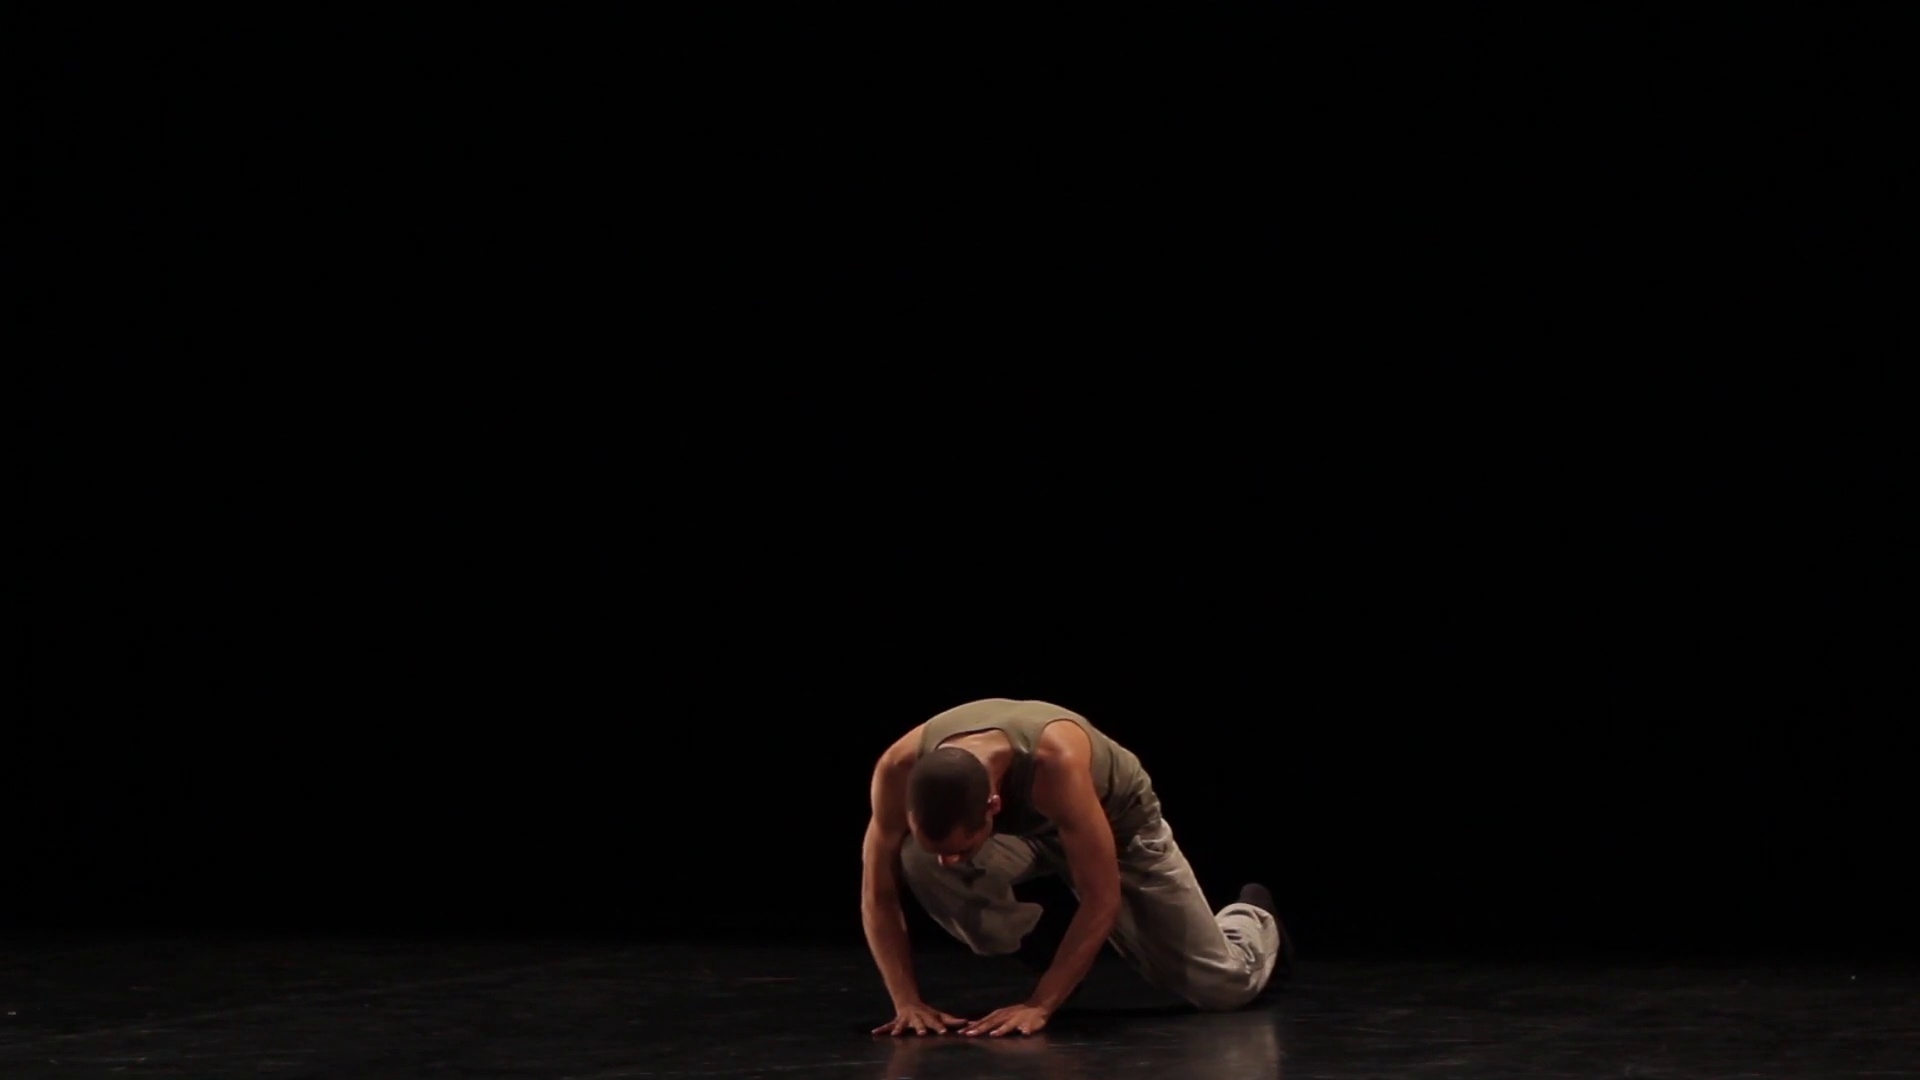
\includegraphics[width=\textwidth]{last_frame_path.jpg}
		\caption{Letzer Frame}
		\label{subfig:lastframe}
	\end{subfigure}
	\begin{subfigure}{0.5\linewidth}
		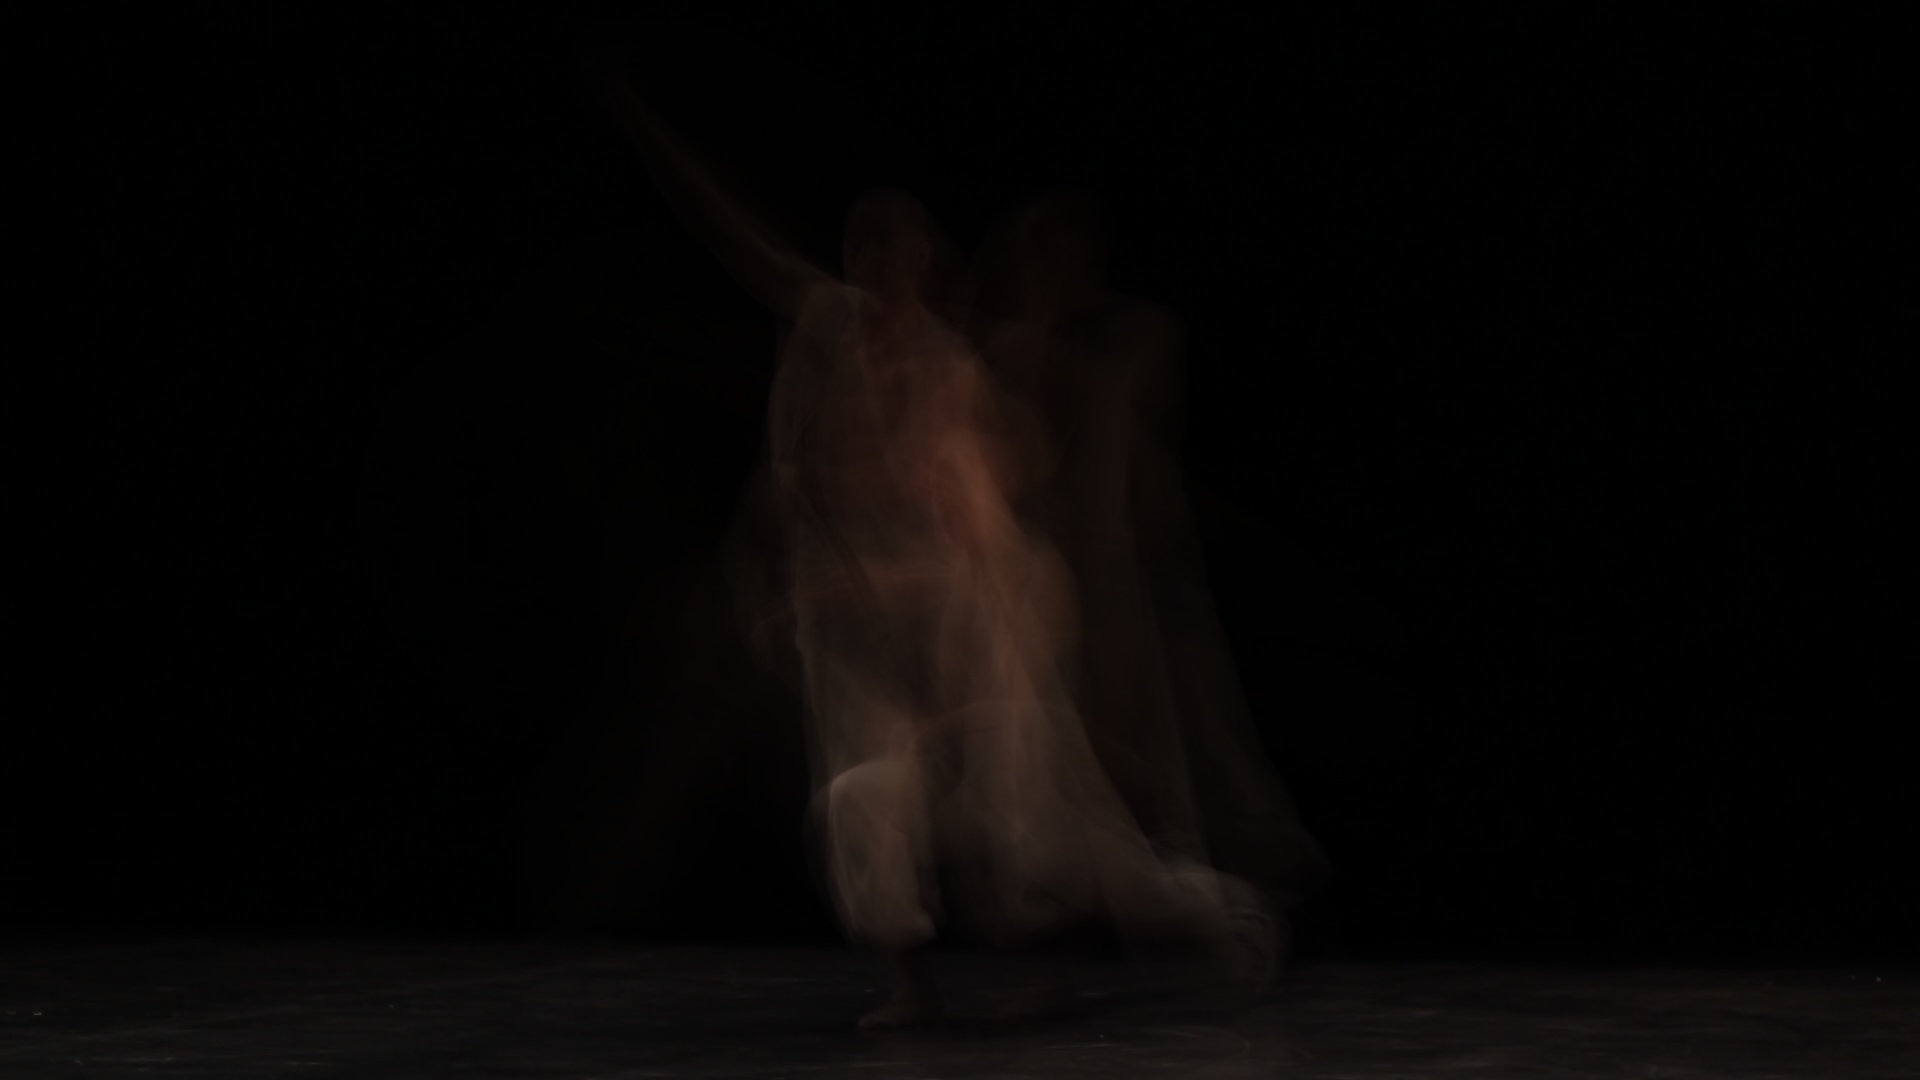
\includegraphics[width=\textwidth]{long_exposure_path.jpg}
		\caption{Langzeitbelichtung}
		\label{subfig:longexposure}
	\end{subfigure}
	\begin{subfigure}{0.5\linewidth}
		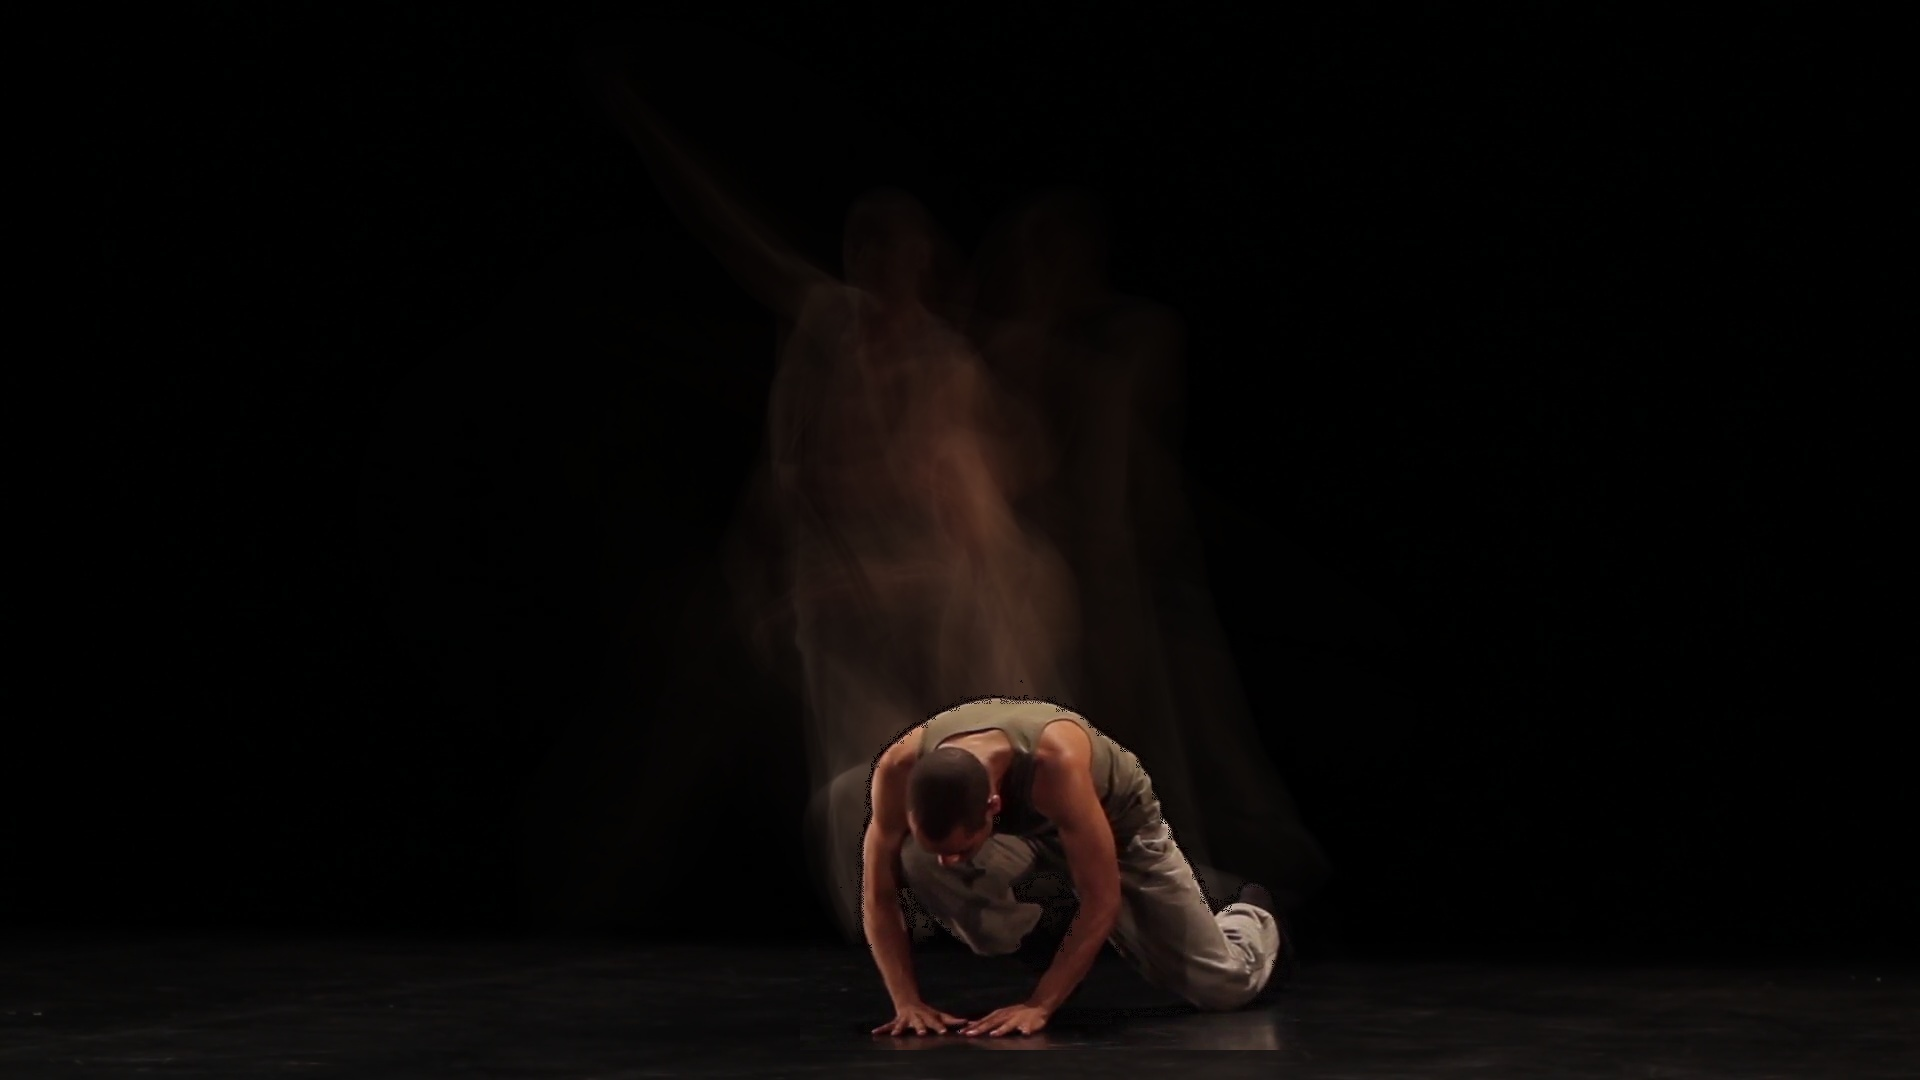
\includegraphics[width=\textwidth]{freeze_me_path.jpg}
		\caption{Langzeitbelichtung + Letzter Frame}
		\label{subfig:grabcutresult}
	\end{subfigure}
	\caption{GrabCut Zwischenschritte und Ergebnis}
	\label{fig:grabcutresultcomplex}
\end{figure}

\section{Edge Detection}
\subsection{Motivation}
Nachdem es der Gruppe gelungen war, Bilder mit einer k\"unstlichen Langzeitblichtung aus dem Video zu erstellen, fiel ein Merkmal auf. Wurde das Video ohne Stativ oder jegliche Art von Unterst\"utzung gedreht, dann f\"uhrte das leichte Wackeln der Kamera irgendwann dazu, dass sich auch stabile Objekte im Ausgabebild als unscharf herausstellten. Um dieses Merkmal oder Problem zu l\"osen, wurde entschieden, Canny Edge Detection zu verwenden.
Die Idee, der Algorithmus zu verwenden, wurde experimentell geboren. Wir haben versucht, Canny Edge Detection auf ein bereits bearbeitetes Bild anzuwenden. Die Methode erkannte nur Objekte als Kanten, die auf dem Video stabil waren. Dann entschied die Gruppe, dass es m\"oglich ist, Sch\"arfungsverfahren $($z. B. einen Laplace-Filter$)$ auf die Pixelkoordinaten mit stabilen Objekten anzuwenden, die mithilfe des Canny Edge Detection auf dem Ausgabebild erhalten werden.
\subsection{Theorie}
%TODOQuelle: https://towardsai.net/p/computer-vision/what-is-a-canny-edge-detection-algorithm
Der Canny Edge Detection ist ein mehrstufiger Algorithmus zum Erkennen von Kanten in einem Bild. Der Algorithmus besteht aus vier Stufen. In der ersten Stufe ist es notwendig, Rauschen aus dem Originalbild zu entfernen, f\"ur diese Aufgabe wird der Gau{\ss} Filter angewendet. Der zweite Stufe besteht darin, den Gr\"o{\ss}e entlang der x- und y-Dimension zu erhalten. Dazu wird die Ableitung des Gau{\ss}-Filters berechnet, um dann das Gradient der Bildpixel zu berechnen.
Der Algorithmus geht alle Punkte der Gradientenintensit\"atsmatrix durch und findet die Pixel mit dem maximalen Wert in den Kantenrichtungen.
Das Betrachten der Gruppe von Nachbarn f\"ur jede Kurve in einer Richtung senkrecht zu der gegebenen Kante unterdr\"uckt nicht maximalen Kantenbeitragspixelpunkte. Schlie{\ss}lich wird das Hysterese-Schwellenwertverfahren verwendet, um die Pixel zu bewahren, die h\"oher als die Gradientengr\"o{\ss}e sind, und diejenigen zu vernachl\"assigen, die niedriger als der niedrige Schwellenwert sind.
\subsection{Codebeschreibung}
Zur Optimierung der Ergebnisse \ref{fig:CED} wird ein Verfahren zur Bestimmung der Schwellwerte $($minVal und maxVal$)$ eingesetzt. Die Schwellwerte werden dann in der OpenCV Methode cv.Canny \"ubergegeben.\\
\subsection{Ergebnis}
\begin{figure}
  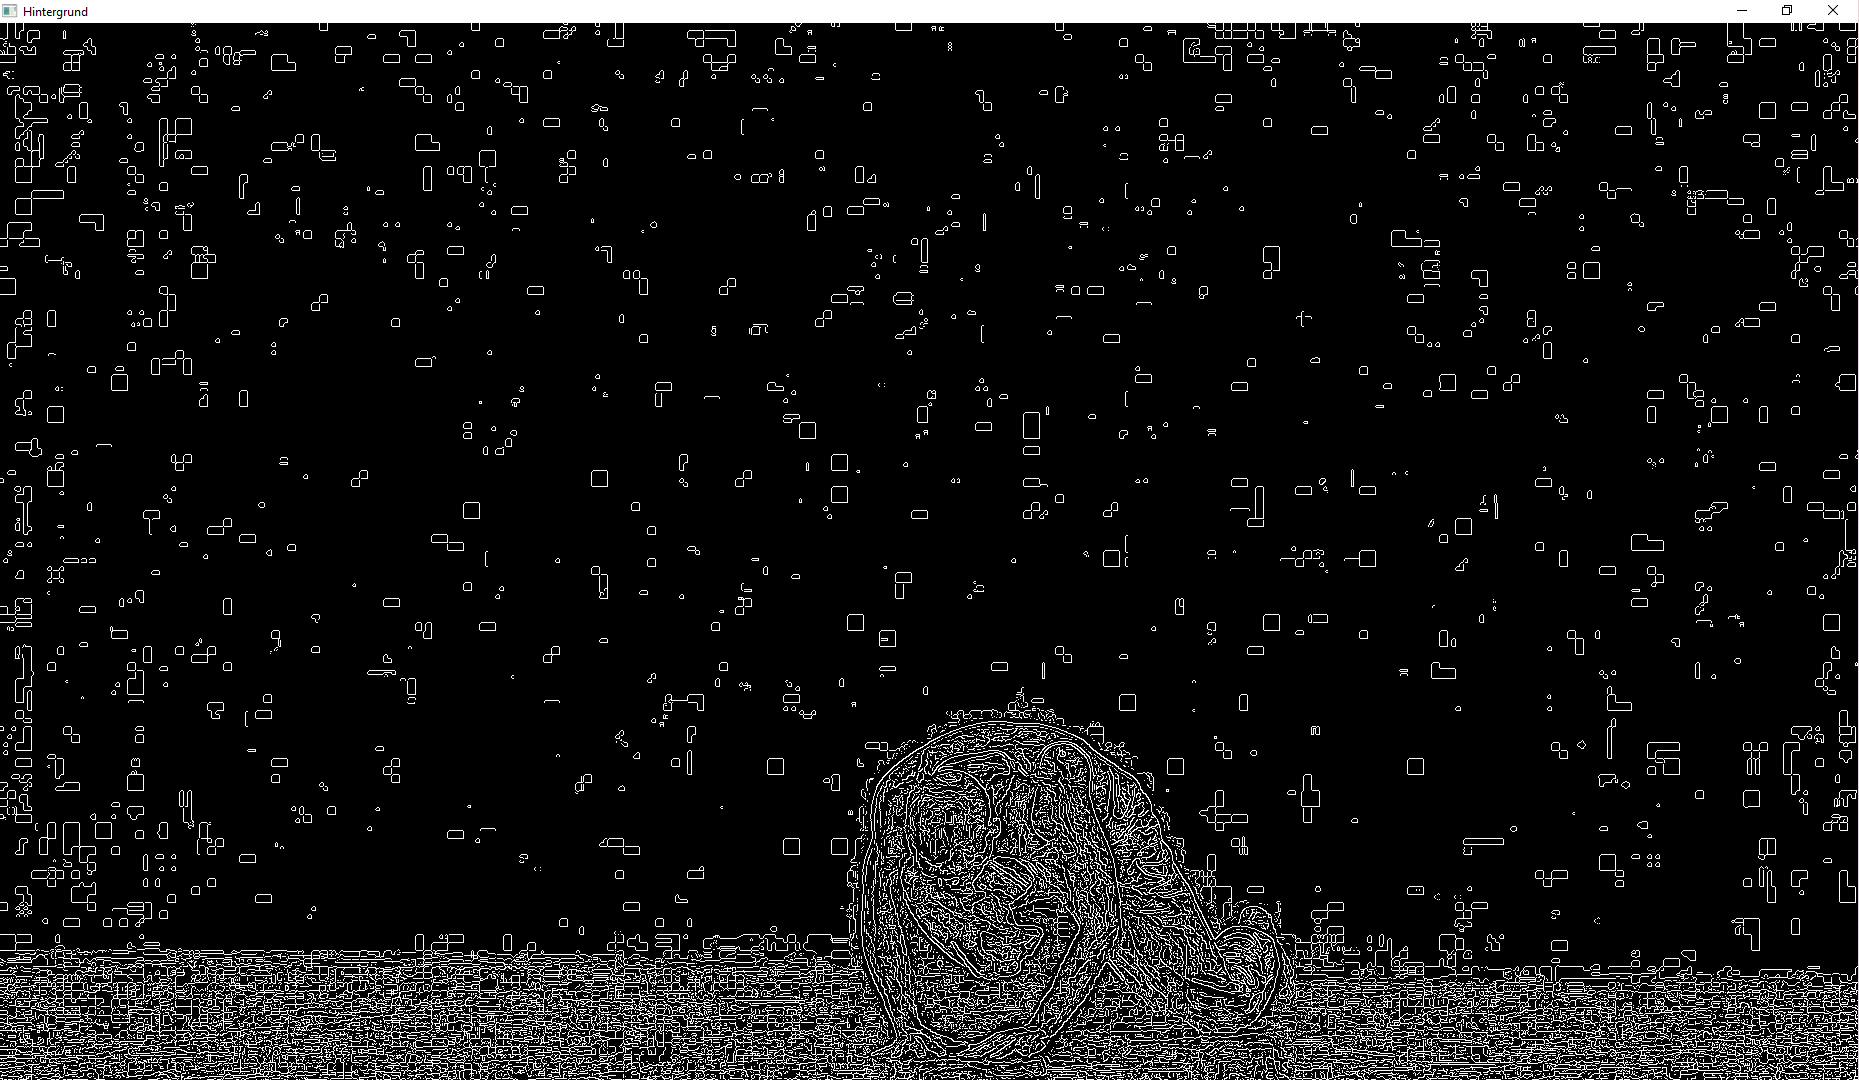
\includegraphics[width=\linewidth]{CED.png}
  \caption{Canny Edge Detection.}
  \label{fig:CED}
\end{figure}
Nach dem Ausf\"uhren des Codes ist das erwartete Ergebnis ein Bild mit identifizierten Kanten. Nach Auswertung der Ergebnisse entschied die Gruppe, dass der resultierende Bildsch\"arfungseffekt nicht effektiv genug war, und entschied sich daher, Canny Edge Detection aufzugeben.\\
\section{Background Subtraction}
\subsection{Motivation}
Die Gruppe stand vor dem Problem, dass manchmal ein sich bewegendes Objekt im Video nach Anwendung der k\"unstlichen Langzeitblichtung weniger unterscheidbar wurde. Um Kontrast und Transparenz hinzuzuf\"ugen, wurde entschieden, dem endg\"ultigen Bild ein sich bewegende Objekt hinzuzuf\"ugen, das aus einem der Videoframes geschnitten wurde.
Zu diesem Zweck entschied sich die Gruppe, zwei Vorder- und Hintergrundsubtraction Methoden von OpenCV anzuwenden:K-Nearest Neighbors $($KNN$)$ und Gaussian Mixture-based $($MOG2$)$.\\
\subsection{Theorie KNN}
%TODOQuelle: https://www.javatpoint.com/k-nearest-neighbor-algorithm-for-machine-learning
Der erste Schritt besteht darin, die Anzahl K der Nachbarn zu w\"ahlen. Dann ist es notwendig, den euklidischen Abstand der Anzahl von K Nachbarn zu berechnen. Basierend auf der berechneten euklidischen euklidischen Distanz werden K n\"achste Nachbarn ausgew\"ahlt. Unter diesen k Nachbarn wird die Anzahl der Datenpunkte in jeder Kategorie gez\"ahlt.
Am Ende werden neue Datenpunkte der Kategorie zugeordnet, f\"ur die die Anzahl der Nachbarn maximal ist.
\subsection{Theorie MOG2}
%TODOQuelle: https://github.com/GuilanITS/mog-motion-detection
Die Mix of Gaussian $($MOG$)$-Hintergrundsubtraktion ist abh\"angig von einer Kombination von Frames anstelle von nur einem Frame. Bei diesem Verfahren wird f\"ur jedes Hintergrundpixel eine Mischung aus einer Gau{\ss}schen Verteilung k und einem Gewichtungsparameter verwendet, um die Lebensdauer von Pixeln in der Szene zu speichern, wobei k im Bereich von 3 bis 5 variieren kann. Verbleibende Pixel mit einer Zeit gr\"o{\ss}er als a Schwellen in der Szene haben eine h\"ohere Wahrscheinlichkeit, zur Hintergrundszene zu geh\"oren. Wenn das Pixel f\"ur einen bestimmten Zeitraum unver\"andert bleibt, wird es als dominantes Hintergrundpixel betrachtet. Wenn die Differenz von Pixeln in einem Frame gr\"o{\ss}er als ein vordefinierter Schwellenwert ist, werden sie als bewegliche Teile klassifiziert. Diese Methode reagiert sehr empfindlich auf Ver\"anderungen in der Umgebung.
In unserem Projekt wird MOG2 verwendet. Der Unterschied besteht darin, dass MOG2 die geeignete Anzahl von Gau{\ss}schen Verteilungen f\"ur jedes Pixel ausw\"ahlt, wobei MOG eine K-Gau{\ss}sche Verteilung f\"ur die Modellierung verwendet. Aus diesem Grund bietet MOG2 eine bessere Anpassungsf\"ahigkeit an wechselnde Szenen aufgrund von Beleuchtungs\"anderungen.
\subsection{Codebeschreibung}
Der Code der Funktion $\glqq$ get\_foreground\_mask$\grqq$ \"uberpr\"uft das Argument $\glqq$foregroundMaskOption$\grqq$, um zu bestimmen, ob die Methode $\glqq$cv.createBackgroundSubtractorMOG2()$\grqq$ oder $\glqq$cv.createBackgroundSubtractorKNN$()$$\grqq$ f\"ur die Hintergrundsubtraktion verwendet werden soll. Der n\"achste Schritt besteht darin, eine URL zum Herunterladen des angegebenen Videos mit videoId und cldId als Parameter zu erstellen. Danach l\"adt es das Video mit urllib.request.urlretrieve() von der URL auf einen lokalen Pfad herunter. Dann wird das VideoCapture-Objekt aus dem heruntergeladenen Video erstellt. F\"ur jeden Frame des Videos wird eine Hintergrundsubtraktion angewendet. Die resultierende Vordergrundmaske wird in einer Datei gespeichert.
Der Code der Funktion $\glqq$get\_background\_image$\grqq$ ist \"ahnlich geschrieben, speichert aber auch Hintergrundbild.\\
\subsection{Ergebnis}
\begin{figure}
  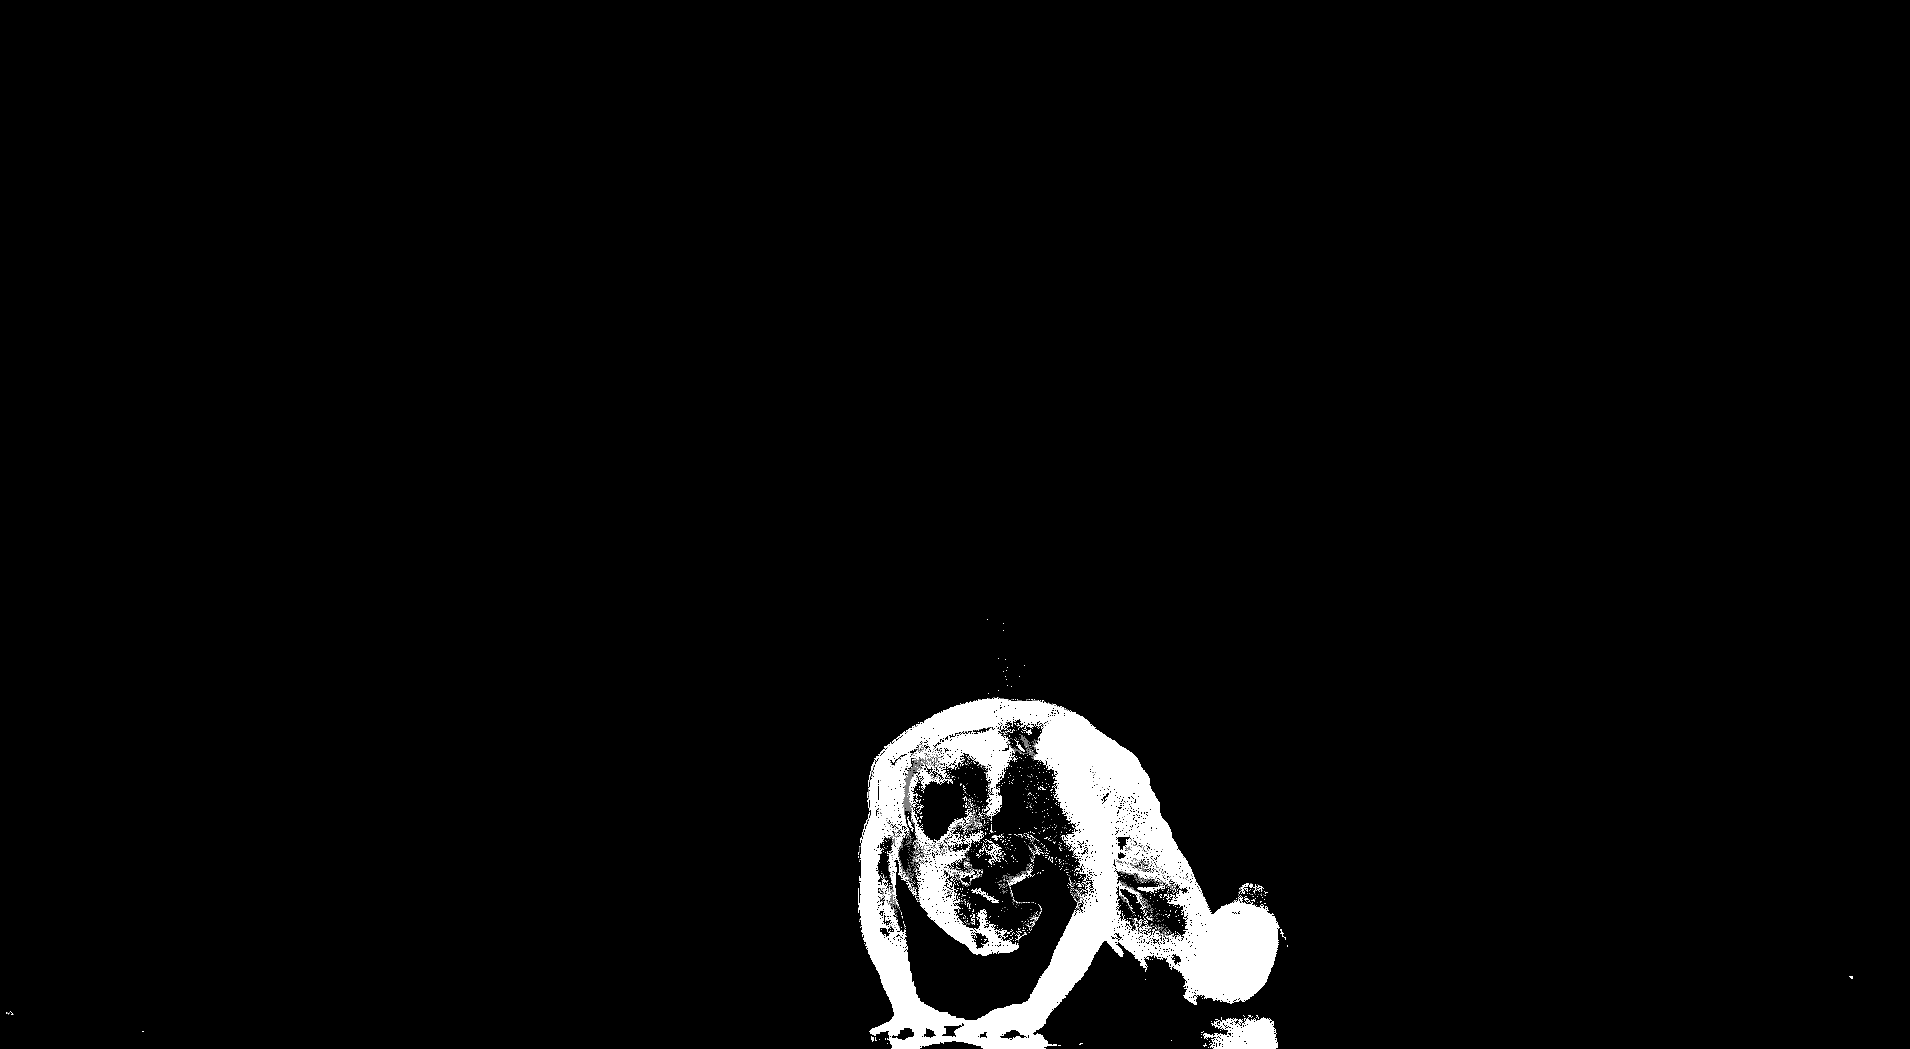
\includegraphics[width=\linewidth]{knn.png}
  \caption{K-Nearest Neighbors.}
  \label{fig:knn}
\end{figure}
Das Ergebnis beider Methoden war f\"ur die Aufgabenstellung nicht geeignet. Die unter Verwendung dieser beiden Algorithmen erhaltenen Masken waren nicht monolithisch, sondern hatten L\"ucken darin. Eine Maske mit L\"ucken war nicht tauglich.
Daher entschied sich die Gruppe f\"ur eine andere Methode f\"ur Hintergrund- und Vordergrundsubtraktion.\\
\begin{figure}
  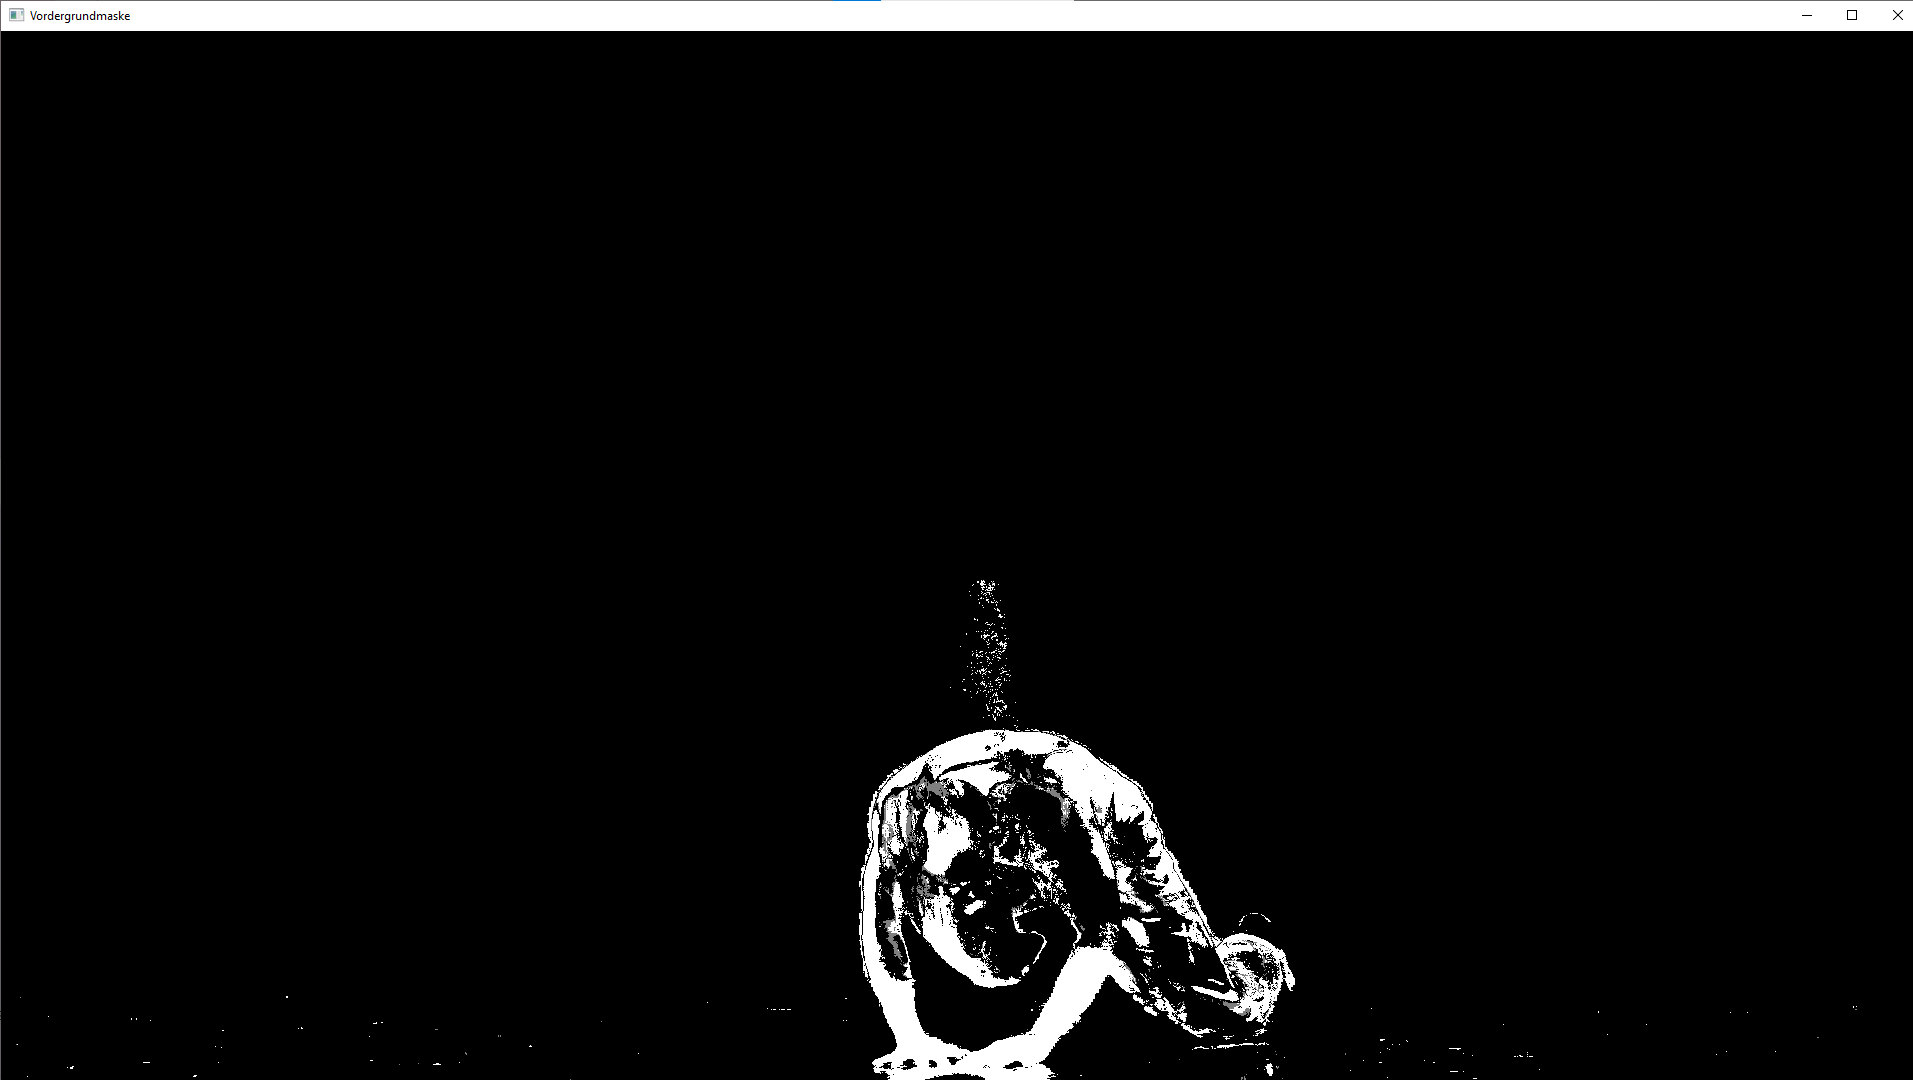
\includegraphics[width=\linewidth]{mog2.png}
  \caption{MOG2}
  \label{fig:mog2}
\end{figure}

\section{Applikation}

Zur Entwicklung einer Applikation, welche die in diesem Projekt geforderte Funktionalit\"at umsetzt, wurde von den Veranstaltern dieser Veranstaltung ein Software Primer bereitgestellt. Dieser Software Primer besteht aus einem Backend und einem Frontend. Das Backend ist eine main.py, welche mit der FastAPI Dependency eine einfache Routing Middleware nutzt und  eine Beispiel-Route implementiert. Das Frontend nutzt das VueJS Framework bereit mit einem initialen Grundger\"ust und Featureimplementationen, wie der Login auf den CEWE Server \"uber deren API. Dar\"uber hinaus ist ein Use-Case implementiert, welcher aufzeigt wie der Frontend-Server mit dem Backend-Server kommuniziert. Wie der Frontend und Backend Server zu starten sind, steht in den README-Dateien der jeweiligen Ordner.

Analog zu dem Beispiel Use-Case aus dem Primer haben wir Kn\"opfe implementiert, welche Videos mit ausgew\"ahlten Methoden auf dem Backend Server transformieren und das Resultat an den Frontend Server zur\"ucksendet. Wir haben den Knopf $\glqq$Extract Background$\grqq$ implementiert, welcher anbei eine Auswahl zwischen zwei Verfahren der background subtraction erlaubt: MOG2 und KNN. Dieser Knopf schickt eine Video-ID und eine Verfahrens-ID an die Backend-Route\\
$\glqq$/get-background-image/\{cldId\}/\{videoId\}/\{backgroundImageOption\}$\grqq$, wo das Verfahren angewandt f\"ur den letzten Videoframe und das Resultat zur\"uck zum Frontend Server gesendet wird, wo das Ergebnis gerendert wird.

Wir haben den Knopf $\glqq$Extract Foreground Mask$\grqq$ implementiert, welcher analog zum Knopf $\glqq$Extract Background$\grqq$ funktioniert, mit dem Unterschied, dass von den vorher gelisteten Verfahren nicht das Hintergrundbild, sondern das Vordergrundbild, zur\"uckgegeben wird. Diese Funktionalit\"at wird bereitgestellt \"uber die Route\\
$\glqq$/get-foreground-mask/\{cldId\}/\{videoId\}/\{foregroundMaskOption\}$\grqq$.

Wir haben den Knopf $\glqq$Extract Edges$\grqq$ implementiert, welche anlaog zu den vorherigen beiden Kn\"opfen funktioniert. Er ermittelt die Kanten des letzten Frames mittels Canny Edge Detection und wird bereitgestellt \"uber die Route\\
$\glqq$/get-edge-detection/\{cldId\}/\{videoId\}$\grqq$.

Der Knopf $\glqq$Apply Long Exposure$\grqq$ implementiert ebenfalls analog eine k\"unstliche Langzeitbelichtung und wird bereitgestellt \"uber die Route\\
$\glqq$/get-long-exposure/\{cldId\}/\{videoId\}$\grqq$.

Zu guter Letzt wird der Knopf $\glqq$Apply Freeze Me$\grqq$ bereitgestellt, welcher die angestrebte Funktionalit\"at des Projekts implementiert. Die Funktionalit\"at wird bereitgestellt \"uber die Route $\glqq$/get-freeze-me/\{cldId\}/\{videoId\}$\grqq$.

% Probleme: Coco Dataset,  HED, Django
\section{Probleme}
\subsection{Coco Dataset}
Die Gruppe versuchte, den Coco-Datensatz zu verwenden, um Objekte zu identifizieren. Es gab jedoch Probleme bei der Installation der Pakete, daher wurde entschieden, diese Methode zu verwerfen.
\subsection{Holistically-Nested Edge Detection $($HED$)$}
Um die Qualit\"at der Kantenerkennung zu verbessern, wurde entschieden, einen Holistically-Nested Edge Detection $($HED$)$ zu verwenden. Das im Youtube Video vorgeschlagene Machine Learning Modell wurde jedoch von seinem Repository entfernt. Daher hat die Methode nicht funktioniert.
\subsection{Django}
Vor der Umstellung auf die Applikation von Cewe wollte die Gruppe eine eigene Anwendung mit Frontend schreiben.

\section{Fazit}
\subsection{Limitierungen}
Die Erkennung des Vordergrundes beschr\"ankt die Funktionsweise der Software in Teilen. Von den anf\"anglich 3 angenommenen Testvideos
$ ( $T\"anzer, Kreuzung, TikTok Sprungvideo$ ) $ funktioniert lediglich der T\"anzer wirklich gut. Das Ergebnis des TikTok Sprungvideos ist
ebenfalls durchaus annehmbar, wobei hier das Hinzuf\"ugen eines maskierten Standbildes weitestgehend wertlos ist. Zu diesem Zwecke m\"usste ein Framepicker in der Software implementiert werden. Gleicherma{\ss}en ist der Kontrast der Hintergrundeffekte relativ stark beschr\"ankt, was ein Betrachten der Resultate in schlechten Lichtverh\"altnissen oder gar auf Beamern stark einschr\"ankt. Um diesen Effekt zu verst\"arken h\"atte eine helligkeitsbedingte Faktorisierung genutzt werden k\"onnen, die wir anf\"anglich mal betrachtet haben, deren Notwendigkeit uns im Laufe des Projektes nicht mehr sinnvoll erschien. Retrospektiv w\"are diese Funktion ein sinniges Opt-In gewesen.
\subsection{Ausbaum\"oglichkeiten}
F\"ur eine k\"unftige Ausgestaltung bieten sich die im letzten Block genannten Optionen an: Eine Optimierung des Interfaces um ein Frame zu selektieren, die Option im entsprechenden Frame ein Rechteck zu w\"ahlen, das dann an GrabCut \"ubergeben wird um den Vordergrund zu bestimmen. Dazu w\"are es eine sicherlich gute Option gewesen die Lichtst\"arke in die Langzeitbelichtung einflie{\ss}en zu lassen, um den Kontrast der Schlieren im Hintergrund zu steigern. Darüber hinaus blieben sicherlich noch Optimierungen an der GUI und der Effizienz und damit der Performanz des Systems.
\subsection{Resumee}
Das letztendliche Ergebnis unserer Arbeit entspricht unser Meinung nach dem urspr\"unglichen Ziel - aufgrund der Subjektivit\"at der
\"Asthetik aber l\"asst sich dieses Urteil wohl kaum objektiv f\"allen. Mit der Anwendung der Langzeitbelichtung fand sich f\"ur uns relativ
fr\"uh eine M\"oglichkeit, einen Hintergrund mit den verwaschenen bzw. verschwommenen Hintergrundartefakten zu erzeugen, durch das Erg\"anzen um ein einzelnes, maskiertes Videoframe ist dabei auch die Charakteristik eines Fotos gewährt.

\end{document}
